%This is my super simple Real Analysis Homework template

\documentclass{article}
\usepackage[utf8]{inputenc}
\usepackage[english]{babel}
\usepackage[]{amsthm} %lets us use \begin{proof}
\usepackage[]{amssymb} %gives us the character \varnothing
\usepackage{amsmath}
\usepackage{hyperref}
\usepackage{colortbl}
\usepackage[usenames,dvipsnames,svgnames,table]{xcolor}
\newcommand\myshade{85}
\colorlet{mylinkcolor}{violet}
\colorlet{mycitecolor}{YellowOrange}
\colorlet{myurlcolor}{Aquamarine}
\hypersetup{
  linkcolor  = mylinkcolor!\myshade!black,
  citecolor  = mycitecolor!\myshade!black,
  urlcolor   = myurlcolor!\myshade!black,
  colorlinks = true,
}
\usepackage{ulem}
\usepackage{tcolorbox}
\usepackage{cancel}
\usepackage{float}
\usepackage{graphics}


\title{Brachistochrone}
\author{Sylvain Vanneste}
\date\today
%This information doesn't actually show up on your document unless you use the maketitle command below

\begin{document}
\maketitle %This command prints the title based on information entered above


\begin{figure}[h]
\begin{center}
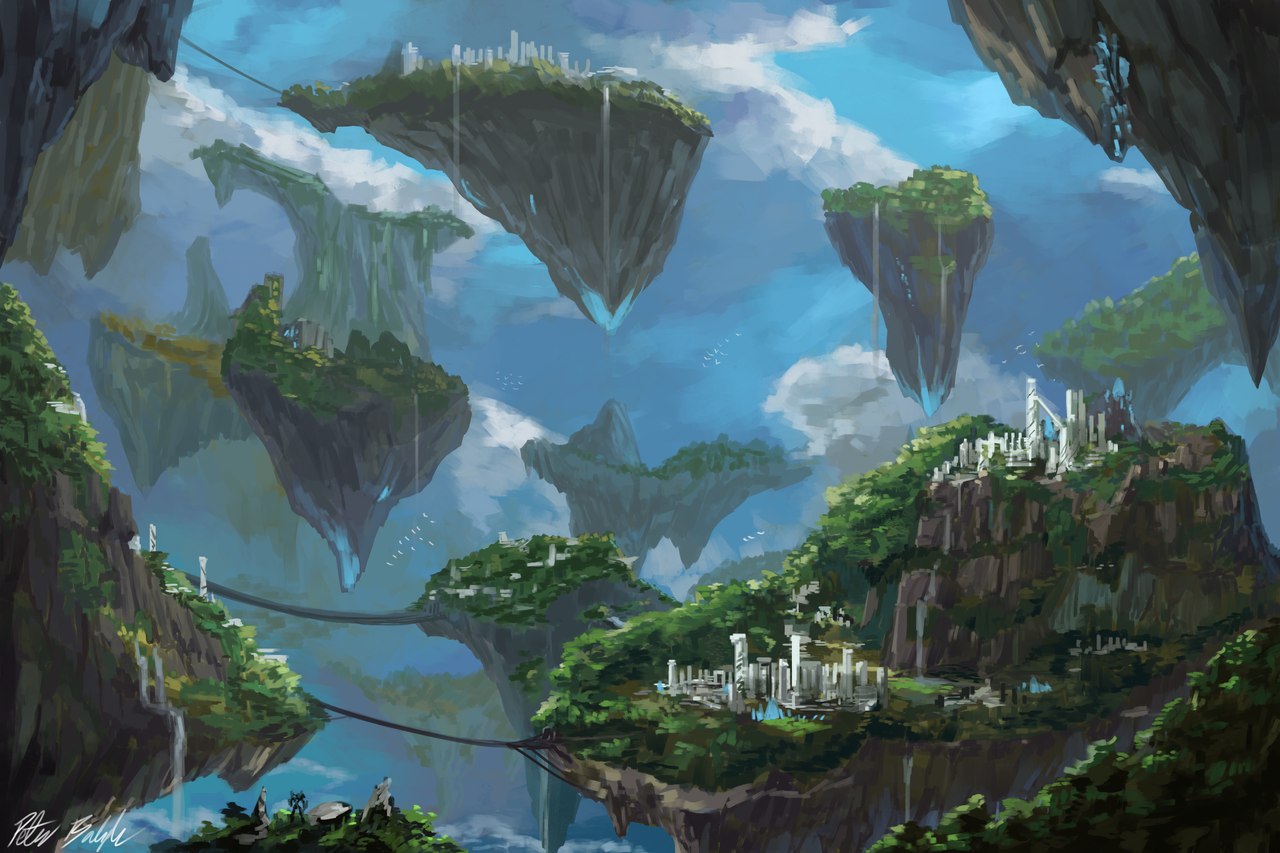
\includegraphics[scale=1.1]{../code/images/FloatingIslands.png}
\end{center}
\caption{Floating Islands by PeterPrime on DeviantArt - 2013}
\end{figure}

\subsection*{Warm up}

Legends say that on an other planet, similar to ours, some cities are built up in the sky. The houses and small neighbourhood are isolated on floating rocks, connected by cables and bridges. Appart from the mysterious mechanism that makes islands fly, the physic there is similar to ours.

Akara lives on one of these floating islands, and she would like to send gifts via a roller-coster to her friend Bun which lives just a little further down on an other island. She built a special tubular structure filled with vacuum and very slippery walls. When a parcel is sent, no initial push is given, and it simply slides down the track under gravity pull, without any friction. However, she would like to know which shape to give to the rail in order to minimise the time a package takes to arrive to her friend.

The situation is picture here after. Akara's house is up left, while Bun's island is down on the right. Three different rails are showed : the first one simply follows a \textit{straight} line; the second adopts a very \textit{steep} curve at the beginning, and flat at the end; and the third a curved path which good \textit{deep} under Bun's island level before going up to its house. As you may have guessed already, the goal is to choose the fastest route... or deduce and build a better one, or even \textit{the best route} ! Does it exist? And if so, does it depends on the mass of the object? Well, answers will follow. But first, as a warm up, let's try to guess if there is a fastest route, and if so, which of the tree paths is the fastest, and why. You can click on the \textit{start/stop} button after you think have a clue.

% animation
\subsubsection*{An intuitive approach}

Well, what do you think about the result? Surprised? Counter-intuitive? Too easy? Probably a bug in the course writer's simulation code? Now, pause a moment, and think why the \textit{steep} is faster than \textit{straight} line, and why the \textit{deep} paths is the fastest. You can use the help of the animation above to observe what's going on.\\

\begin{tcolorbox}

\paragraph{Hints and solution}
\begin{itemize}
  \item A bit of physics will help understand what is happening here. Intuitively, we can see that as a package descends, it gains speed. The lower it is in relation to Akara's house, the faster it goes along the rail.
  \item Although the \textit{straight} line is the \textit{shortest} distant, is it by far the slowest. The trajectory a rough compromise between going toward Bun's house and going down to gain speed, and clearly, success is not there. The package looses too much time at the beginning.
  \item On the contrary, the first instants on the \textit{steep} curve are spent going down as fast as possible to gain speed, then use these speed to go right and reach destination.
  \item Finally, the \textit{deep} curve chooses to go rather deeply, maximising the velocity for a moment, before reaching Bun's island. This last approach is actually the fastest.
\end{itemize}
\end{tcolorbox}
~

We have our intuitive solution! The curve which is the fastest should find a compromise between reaching high speed by going down, while still spending some time going to the right.

This is only the beginning of the story. Believe it or not, Akaras's questioning is a famous problem in physics which leads to beautiful and multiple theoretical and experimental demonstration.

\subsubsection*{A challenge for the brightest}

This challenge was proposed to mathematicians by Johann Bernoulli in June 1696 in a straighter form :
\begin{center}
  \textit{Given two points A and B in a vertical plane, what is the curve traced out by a point acted on only by gravity, which starts at A and reaches B in the shortest time.}
\end{center}
Such curve are was labelled \textit{Brachistochrone}, meaning 'shortest time' from Ancient Greek. For the record, according to Newton's niece, Catherine Conduitt, Newton red the letter of Johann Bernoulli on January 1697, and found a solution in late in that night. In the following, we will discover some approaches which solve this problem in a beautiful way.


\subsubsection*{What do matters, what doesn't}

Enough talking, here is a second question for you : is the mass of the package important for the path design of the rails? (remember, we can neglect all loss of speed due to friction).

The answer is immediate if you know a bit of Galileo's work. It is even considered as the first law of modern physics :\\

\begin{tcolorbox}
\begin{center}
  \textit{In the vacuum, the speed of an object in free fall is independent of its mass}
\end{center}
\end{tcolorbox}
~

Well, it looks like this is the case for us, no vertical frictions is some kind of free fall, right?

Mathematically, a similar conclusion arises when considering one of the fundamental postulate of modern physics : energy conservation. Knowing that the energy a package has is constant along the rails, and that it is equal to the sum of its kinetic and potential energy, $E_k$ and $E_p$ respectively, can you show why the speed $v$ at anytime during the descent does not depend on its mass $m$, and depends only on the height $y$ of the parcel from the ground? (well supposed there is a ground of course, nobody ever saw it from the city, many legends exists...)

\begin{tcolorbox}

\paragraph{Hints and steps of the solution}

\begin{enumerate}

\item In physics, the concept of an object \text{energy} is very abstract. It serves to quantify the capability of this object to do some \textit{work}. Well, what is \textit{work}? It is a slightly less abstract quantity, which pictures the process of converting this energy into motion via application of a force (the snake probably slightly bites its tail here). A simple example is the potential energy of a trebuchet. As the counter-weights are manually levered, they accumulate potential energy. When the weights are released, they briefly transfer all their energy into the projectile via the trebuchet arm. The projectile undergo a huge force, which accelerate it. Some of the initial potential energy of the weights are now present in the form of kinetic energy for the projectile. The rest of the energy is transferred elsewhere during the shot via frictions and heat.

\item The kinetic energy reads $E_k=m v^2/2$, while the potential $E_p=m g y$, where $g\simeq 10 \,\text{m/s}^2$ is the free fall acceleration of any object on this planet (considered as constant locally). Now remember the postulate of energy conservation : the parcel \textit{total} energy (potential+kinetic) is constant along the rail. Therefore, if as it looses some potential energy, it should acquire equivalently some kinetic energy.

% \item Remember that nobody has ever see the ground? Well then, what is the heigh $y$ in that case? Simple, choose it! Let choose Akara's house as the ground, such that the initial heigh is zero,  $y=0$.


\item The key is to write the total energy at any time :
\begin{align}
E &= E_k + E_p\nonumber\\
&= \frac 12  mv^2 + m g y.\nonumber
\end{align}
Now, write down and simplify the initial energy $E_i$ of the parcel when it has not yet moved from Akara's island (located at height $y_A$), with the energy of the parcel when it is anywhere else, $E$.

\item Applying as suggested above,
\begin{align}
E_i &= E_{k,i} + E_{p,i}  = 0 + mgy_A ~~\text{(initial kinetic energy is null.)}\nonumber\\
E &= E_{k} + E_{p} = \frac 12  mv^2 + m g y ~~\text{(total energy when anywhere else)}\nonumber\\
\rightarrow E &= E_i \nonumber~~\text{(energy conservation)} \\
\Leftrightarrow~& \frac 12  \cancel{m}v^2 + \cancel{m} g y = \cancel{m}gy_i~~\text{(all mass terms cancel out !)}\nonumber \\
\Leftrightarrow~& v = \sqrt{g (y - y_A)}\nonumber\\
\Leftrightarrow~& \boxed{v(y) = \sqrt{g \Delta y}}\nonumber ~~\text{with $\Delta y=y - y_A$, the distance from A's house}
\end{align}

\end{enumerate}
\end{tcolorbox}
~

That's right! From energy conservation, we deduce not only that the velocity in vacuum free fall does not depend on the mass $m$, but also that it is proportional to the square root of the distance from Akara's house. We can express it as a function of time the height $y$
\begin{align}
  \boxed{v(y) = \sqrt{g (y - y_A)}}
\end{align}
Okay, this not only confirms our intuition, but provides an exact relation between speed and height as well. In addition, we make an important observation here : the motion speed of the body in free fall along an arbitrary curve does not depend on the horizontal displacement.

\subsubsection*{next}




Now what do we do next?


- Can you find a solution of the brachistochrone that time-minimizing curve is represented by a straight line in theta-t plot.

- Tautochrone


\subsubsection*{next}

\newpage
\section*{Personal notes}

We want to minimise the time it take for an object to goes from $A$ to $B$, $t_{AB}$. We define $v$ as the speed of the object, $g$ the gravitational constant, and $m$ the object's mass. The trajectory of the object can be defined by relation between its horizontal and vertical position, $y = f(x)$. For simplicity, we will write $y = y(x) = f(x)$.

Using energy conservation, we have
\begin{align}
  &E_{\text p} + E_{\text c} = E_{\text{pi}} + E_{\text{ci}}\nonumber\\
\Leftrightarrow~ & mgy + \frac 12 m v^2 = mgy_A + 0\nonumber\\
\Leftrightarrow~& v(y) = \sqrt{2 g(y_A - y)}, \label{eq:vtoy}
\end{align}
where $v(y)$ is a function of the object heigh $y$.

The time $t_{AP}$ for the object to go from point $A$ to an arbitrary position $P$, with $P\in[A, B]$, is written
\begin{align}
t_{AP} = \int \frac{\text d s }{v(y)}, \label{timeAP}
\end{align}
with $\text d s $ the infinitesimal distance increment of the object. It can be expressed using Pythagorean law
\begin{align}
\text d s^2  &= \text d x^2 + \text d y^2 \nonumber\\
\Leftrightarrow~ \text d s &= \sqrt{1 + \frac{\text d y^2}{\text d x^2}}\text d x\nonumber\\
 & = \sqrt{1 + y'^2}\text d x,\label{eq:dstodx}
\end{align}
where the derivative of the function is written $y' = \text d y/\text d x = f(x)'$.

Using Eqs. \eqref{eq:vtoy} and \eqref{eq:dstodx}, we can now simplify the time Eq. \eqref{timeAP},
\begin{align}
t_{AP} &= \int_A^P \frac{\text d s }{v(y)},\nonumber\\
&= \int_{x_A}^{x_P} \frac{\sqrt{1 + y'^2(x)}}{\sqrt{2 g(y_A - y(x))}} \text d x,\nonumber\\
&= \frac 1{\sqrt{2 g}} \int_{x_A}^{x_P} \frac{\sqrt{1 + y'^2(x)}}{\sqrt{(y_A - y(x))}} \text d x, \label{eq:tAP}
\end{align}

Therefore, the time $t_{AB}$ the object takes to go from point $A$ to $B$ is depends on the trajectory $y(x)$. Seeking a minimising this time is equivalent to seek for a function $y(x)$ which minimise the Eq. \eqref{eq:tAP} (where $x_P = x_B$).

Before seeking for such solution, we first compare the physical behaviour for some known functions $y(x)$, namely : the straight line, the reciprocal function, and a second order polynomial function.

\subsection*{The straight line}

The straight line between point $A$ and $B$ can be expressed as
\begin{align}
y = \alpha x + \beta,
\end{align}
where $\alpha = (y_B-y_A)/(x_B - x_A)$ and $\beta = y_A - \alpha x_A$. The function derivative is therefore $y' = \alpha$, and the time for an object to reach a point $P$ is written
\begin{align}
t(x) &= \frac 1{\sqrt{2 g}} \int_{x_A}^{x_P} \frac{\sqrt{1 + y'^2(x)}}{\sqrt{(y_A - y(x))}} \text d x,\nonumber\\
&= \frac 1{\sqrt{2 g}} \int_{x_A}^{x_P} \frac{\sqrt{1 + \alpha^2}}{\sqrt{y_A - \alpha x - \beta }} \text d x,\nonumber\\
&=  \sqrt{\frac{1 + \alpha^2}{2 g}} \int_{x_A}^{x_P} \frac{1}{\sqrt{y_A - \alpha x - \beta }} \text d x,\nonumber\\
&=  - \sqrt{\frac{1 + \alpha^2}{2 g}} \frac 2 \alpha \left[ \sqrt{y_A - \alpha x - \beta }  \right]_{x_A}^{x_P},\nonumber\\
&=  - \sqrt{\frac{1 + \alpha^2}{2 g}} \frac 2 \alpha \left[ \sqrt{y_A - \alpha x_P - \beta } - \sqrt{y_A - \alpha x_A - \beta }  \right]\label{eq:tAP_straight}
\end{align}

Conversely, the position $x_P$ can be written as a function of the time,
\begin{align}
x_P(t) = -\frac 1 \alpha \left [ \left(- t \frac{\alpha}{2} \sqrt{\frac{2g}{1 + \alpha^2}} + \sqrt{-\alpha x_A- \beta + y_A}\right)^2 - \beta + y_A \right].
\end{align}

\subsection*{The reciprocal function}

We now choose the reciprocal function
\begin{align}
y(x) = \frac1{x+\gamma} + \eta,
\end{align}
therefore $y'(x) = -(x+\gamma)^{-2}$.

Since $x_A = 0$ and $y_A=0$, we have $\eta = -1/\gamma$, and $\displaystyle \gamma = \pm\frac{\sqrt{x_B} \sqrt{- x_B y_B + 4}}{2\sqrt{x_B}} - \frac{x_B}2$. We choose the $+$ sign for the second condition in order for $y(x)$ to be convex.

The time for an object to reach a point $P$ is computed by numerical integration, following
\begin{align}
t(x) &= \frac 1{\sqrt{2 g}} \int_{x_A}^{x_P} \frac{\sqrt{1 + y'^2(x)}}{\sqrt{(y_A - y(x))}} \text d x.\\
\label{eq:tAP_reciprocal}
\end{align}

\subsection*{2nd order polynomial function}

We now choose a 2nd order polynomial function of the form
\begin{align}
y(x) = a x^2 + b x + c,
\end{align}
with the condition $y(x) \leq y_A$. Therefore $y'(x) = 2a + b$. We also choose $y(x)$ to be convex, therefore $y(x)'' \geq 0$, which leads to $a \geq 0$. Since $x_A = 0$ and $y_A=0$, we have $c=0$. Finally, $b = y_B - a x_B^2$.


\subsection*{Cycloid}

Equation of motions are
\begin{align}
  x(r, \phi) &= r(\phi - \sin(\phi))\\
  y(r, \phi) &= r(1 - \cos(\phi))
\end{align}
the parameter $r$ is the radius of the rotating cycle along the horizontal axis passing thought $x_A$, while $\phi$ its angle of rotation (starting at $x_A$). The value of $\Phi$ is computed by numerically solving the equation,
\begin{align}
  \frac{x_B}{y_B} = \frac{\Phi - \sin{\Phi}}{1 - \cos{\Phi}},
\end{align}
while the radius is computed using $r=x_B/(\Phi - \sin(\Phi))$.

From Fermat’s minimum time principle, we have
\begin{align}
  \frac{dx}{ds} = \frac{v}{v_m},
\end{align}
with $v_m = 2\sqrt{gr}$ the maximum speed, at the bottom of the curve, when $y=2r$. Therefore, the time function is given by
\begin{align}
  t &= \int_{A}^{B} \frac{ds}{v}\\
  & = v_m \int_{A}^{B} \frac{dx}{v^2}\\
  & = v_m \int_{A}^{B} \frac{dx}{2 gy}\\
  & = v_m \int_{0}^{\phi} \frac{r(1 - \cos(\phi))}{2 gr(1-\cos(\phi))}d\phi\\
  & = \phi \sqrt{\frac rg}.
\end{align}

All three functions $x, y, t$, are interpolated by varying $\phi\in [0,\Phi]$, where $\Phi$ is the angle of rotation when $x=x_B$.


\section*{Refs}

% - Solving a Non-Existent Unsolved Problem: The Critical Brachistochrone : \href{http://klotza.blogspot.com/2015/08/the-critical-brachistochrone-solving.html}
% - problems : \href{http://www.dam.brown.edu/people/jgemmer/brachistochrone.html}
% - parametrisation :  \href{https://proofwiki.org/wiki/Equation_of_Cycloid_in_Cartesian_Coordinates}
% vieux site : https://mathcurve.com/courbes2d.gb/brachistochrone/brachistochrone.shtml
% - https://mathcurve.com/courbes2d.gb/brachistochrone/bachistodelongueurfixe.shtml

\end{document}
